\documentclass{ximera}
\title{Newton's Methods}
\begin{abstract}
\end{abstract}
\begin{document}
\maketitle
\section{Introduction}
\begin{dialogue}
\item[Dylan] I'm so tired of having to solve roots by hand. It's a real drag.
\item[Julia] Yeah, some of these roots are rough. I wish there was a better way!
\item[James] There's always a better way!
\item[Dylan and Julia] Show us!!!
\item[James] Maybe you've heard of Sir Isaac Newton? He got tired of solving roots too, and made a whole method to approximate them!
\item[Dylan] Wow! I'm just like him except worse in every way!
\end{dialogue}
Newton's Method is a system of approximating roots of polynomials by using tangent lines from an initial estimate. While this method is extremely accurate when used properly, it is possible to have a very inaccurate estimate when used improperly.
\section{Guided Example}
In the following figure we have an initial guess $x_{0}$, then we have the blue tangent line with respect to the point $x_{0}$
\begin{image}
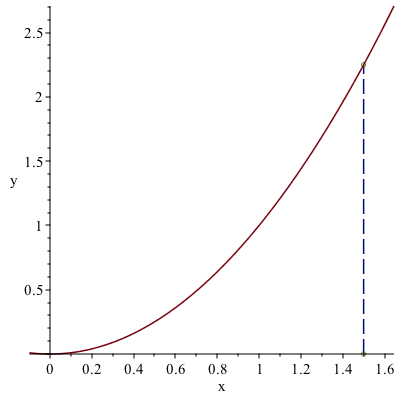
\includegraphics{NewtonMethod}
\end{image}
\begin{question}

What is the slope, in general, for the tangent line of $y=f(x)$ at $x_{0}$?

\begin{multipleChoice}
\choice[correct]{$f'(x_0)$}
\choice{$f'(x)$}
\choice{$f(x)$}
\choice{$f(f(x))$}
\end{multipleChoice}

What is the equation of the tangent line for the point $(x_{0},f(x_{0})$?

\begin{multipleChoice}
\choice{$y=f(x) \cdot x + f(x_0)$}
\choice[correct]{$y = f'(x_0)\cdot (x-x_0)+f(x_0)$}
\choice{$y = f'(x) \cdot b + x_0$}
\choice{$y = f'(x) \cdot b + f(x)$}
\end{multipleChoice}

How would you use the tangent line you found above to estimate the value of the root?

\begin{multipleChoice}
\choice{Solve for $x=0$ to find a point near the actual root.}
\choice[correct]{Solve for $y=0$ to find a point near the actual root.}
\choice{Take the derivative of the tangent line to find where the second derivative is zero.}
\choice{Evaluate the tangent line at a $y$-value which was the initial estimate.}
\end{multipleChoice}

\end{question}
\section{On Your Own}
\begin{question}
Consider the function $f(x) = x^2-1$.
\[
\graph{x^2-1}
\]

Find the equation of the tangent line at an initial estimate of $x_0=3$.

$y = \answer{6x-10}$

Plot the tangent line and function on the same axes. Does the x-intercept of the tangent line seem more or less accurate than your initial estimate?

\begin{multipleChoice}
\choice[correct]{More Accurate}
\choice{Less Accurate}
\end{multipleChoice}

What is the x-intercept of the tangent line?

$\answer{\frac{5}{3}}$
\begin{onlineOnly}
\begin{sageCell}

\end{sageCell}
\end{onlineOnly}
Continue this process until the x-intercepts change by less than .0001 on each iteration. How many iterations did this take?

$\answer{5}$
\end{question}
\begin{question}
Consider the function $g(x) = x^3-4x^2-1$.
\[
\graph{x^3-4x^2-1}
\]
Why does $g(x)=0$ have only one solution? Explain with the help of a graph.

\begin{freeResponse}
\end{freeResponse}
\end{question}

Fortunately, with the use of Sage Cells, we don't have to do all of this by hand! The following Sage Cell contains the commands through which we can perform Newton's Method, along with comments explaining just what it is that Sage is doing.

\begin{onlineOnly}
\begin{sageCell}
x = var('x')#This line declares the variable we will be using
f(x)=cos(x)+5*x-5#Here we define the function whose root we're estimating
df=diff(f,x)#We then find the derivative of the function
NewtonsMethod(x)=x-(f/df)(x)#The formula for Newton's Method, which we are calling "NewtonsMethod"
x0=1# initial guess
print x0#displays the initial guess in the output
x1=N(NewtonsMethod(x0))#first iteration of the method
print x1#displays first result
x2=N(NewtonsMethod(x1))#second iteration of Newtons Method
print x2#displays second result
\end{sageCell}
\end{onlineOnly}

The only way to run Newton's Method like this will be to take the first few lines of code and put them in each cell after this - the method is \textbf{not} defined as a function in Sage.

\begin{question}
Using $g(x) = x^3 -4x^2-1$ from before, use an initial guess of 2. After 5 iterations, what result do you get?

\begin{onlineOnly}
\begin{sageCell}

\end{sageCell}
\end{onlineOnly}

$\answer[tolerance=0.001]{-0.395459530414480}$

Why is it important to use caution with your first guess when doing Newton's Method by hand? It might help you to understand why if you plot both the function and the tangent lines from Newton's method in the following Desmos graph.

\[
\graph{}
\]

\begin{freeResponse}
\end{freeResponse}
\end{question}

\begin{question}
Consider the function $h(x) = 4x^3 - 12x^2 + 2x + 1$.
\[
\graph[xmin=-6,xmax=6,ymin=-15,ymax=7,height=400]{4x^3 - 12x^2 + 2x + 1}
\]
\begin{onlineOnly}
\begin{sageCell}

\end{sageCell}
\end{onlineOnly}


Use an initial guess of $x=3$ to estimate a root of $h(x)$. What did you get after the fifth iteration?

$\answer[tolerance=0.01]{2.78854472256823}$

Look at the graph, and attempt to estimate another root using $x = 0$. Did you find the root to the right or the left of this point?

\begin{multipleChoice}
\choice[correct]{Left}
\choice{Right}
\end{multipleChoice}

Increment the $x$ guess by $0.02$ and use Newton's method until you find the root on the right. What value of $x$ is the first to work?

\begin{onlineOnly}
\begin{sageCell}

\end{sageCell}
\end{onlineOnly}

$\answer{0.1}$
\end{question}

\section{In Summary}
\begin{dialogue}
\item[Julia] Wow! Newton's Method is awesome!
\item[Dylan] Yeah, it's way more accurate than just guessing! If you're too far off on that initial guess though...
\item[James] Things can go downhill quickly. While Newton's Method can be handy, it's important to remember how important an accurate initial estimate is!
\item[Dylan and Julia] Thanks James!
\end{dialogue}
\end{document}